\documentclass[tikz,border=8pt]{standalone}
% Shared look for every TikZ diagram. Load with % Shared look for every TikZ diagram. Load with % Shared look for every TikZ diagram. Load with \input{../../tools/tikz-style.tex}
\usepackage[T1]{fontenc}
\usepackage{lmodern}
\renewcommand{\sfdefault}{lmr}  % diagrams use the same serif as the text
\usetikzlibrary{arrows.meta, positioning, shapes.geometric, calc, fit, backgrounds}
\definecolor{cblue}{HTML}{4C78A8}
\definecolor{corange}{HTML}{F58518}
\definecolor{cgreen}{HTML}{54A24B}
\definecolor{cred}{HTML}{E45756}
\definecolor{cpurple}{HTML}{B279A2}
\definecolor{cgrey}{HTML}{6B6B6B}
\tikzset{
  every picture/.style={font=\sffamily, line width=1.2pt},
  box/.style={draw=#1, fill=#1!12, rounded corners=4pt, align=center, inner sep=7pt, minimum height=1.1cm},
  box/.default=cgrey,
  arrow/.style={-{Stealth[length=3mm]}, draw=cgrey, line width=1.4pt},
  title/.style={font=\sffamily\bfseries\Large},
  note/.style={font=\sffamily\small, text=cgrey, align=center},
}
\AtBeginDocument{\hyphenpenalty=10000 \exhyphenpenalty=10000}

\usepackage[T1]{fontenc}
\usepackage{lmodern}
\renewcommand{\sfdefault}{lmr}  % diagrams use the same serif as the text
\usetikzlibrary{arrows.meta, positioning, shapes.geometric, calc, fit, backgrounds}
\definecolor{cblue}{HTML}{4C78A8}
\definecolor{corange}{HTML}{F58518}
\definecolor{cgreen}{HTML}{54A24B}
\definecolor{cred}{HTML}{E45756}
\definecolor{cpurple}{HTML}{B279A2}
\definecolor{cgrey}{HTML}{6B6B6B}
\tikzset{
  every picture/.style={font=\sffamily, line width=1.2pt},
  box/.style={draw=#1, fill=#1!12, rounded corners=4pt, align=center, inner sep=7pt, minimum height=1.1cm},
  box/.default=cgrey,
  arrow/.style={-{Stealth[length=3mm]}, draw=cgrey, line width=1.4pt},
  title/.style={font=\sffamily\bfseries\Large},
  note/.style={font=\sffamily\small, text=cgrey, align=center},
}
\AtBeginDocument{\hyphenpenalty=10000 \exhyphenpenalty=10000}

\usepackage[T1]{fontenc}
\usepackage{lmodern}
\renewcommand{\sfdefault}{lmr}  % diagrams use the same serif as the text
\usetikzlibrary{arrows.meta, positioning, shapes.geometric, calc, fit, backgrounds}
\definecolor{cblue}{HTML}{4C78A8}
\definecolor{corange}{HTML}{F58518}
\definecolor{cgreen}{HTML}{54A24B}
\definecolor{cred}{HTML}{E45756}
\definecolor{cpurple}{HTML}{B279A2}
\definecolor{cgrey}{HTML}{6B6B6B}
\tikzset{
  every picture/.style={font=\sffamily, line width=1.2pt},
  box/.style={draw=#1, fill=#1!12, rounded corners=4pt, align=center, inner sep=7pt, minimum height=1.1cm},
  box/.default=cgrey,
  arrow/.style={-{Stealth[length=3mm]}, draw=cgrey, line width=1.4pt},
  title/.style={font=\sffamily\bfseries\Large},
  note/.style={font=\sffamily\small, text=cgrey, align=center},
}
\AtBeginDocument{\hyphenpenalty=10000 \exhyphenpenalty=10000}

\begin{document}
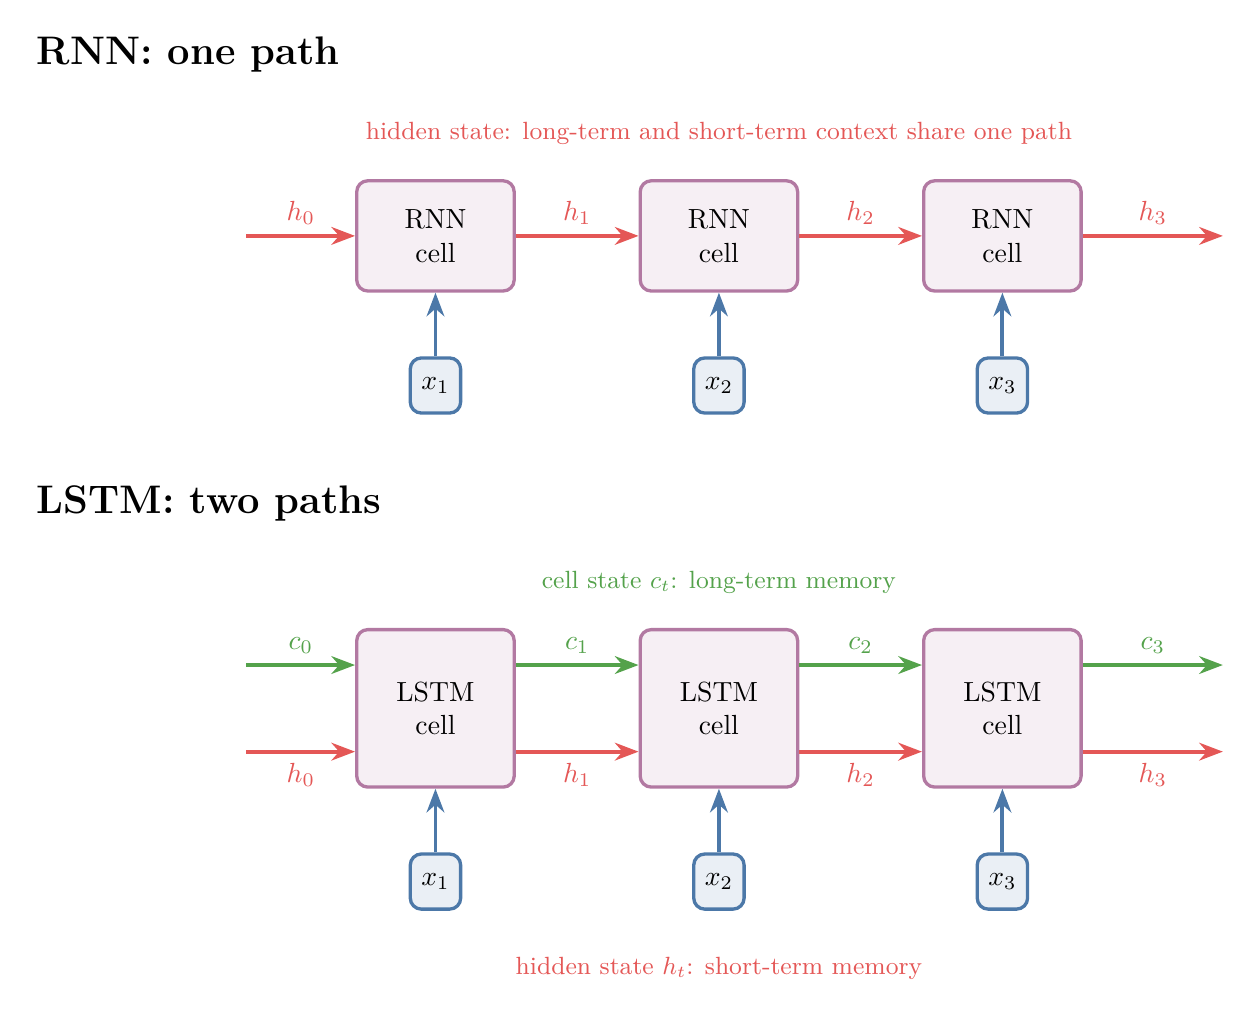
\begin{tikzpicture}[cell/.style={box=cpurple, minimum width=2.0cm, minimum height=1.4cm}]
  % RNN row
  \node[title, anchor=west] at (-1.6,2.3) {RNN: one path};
  \foreach \t in {1,2,3} {
    \node[cell] (r\t) at (3.6*\t,0) {RNN\\cell};
    \node[box=cblue, minimum height=0.7cm, inner sep=4pt] (rx\t) at (3.6*\t,-1.9) {$x_{\t}$};
    \draw[arrow, draw=cblue] (rx\t) -- (r\t);
  }
  \draw[arrow, draw=cred] (1.2,0) -- node[above, text=cred] {$h_0$} (r1);
  \draw[arrow, draw=cred] (r1) -- node[above, text=cred] {$h_1$} (r2);
  \draw[arrow, draw=cred] (r2) -- node[above, text=cred] {$h_2$} (r3);
  \draw[arrow, draw=cred] (r3) -- node[above, text=cred] {$h_3$} (13.6,0);
  \node[note, text=cred] at (7.2,1.3) {hidden state: long-term and short-term context share one path};
  % LSTM row
  \begin{scope}[yshift=-6cm]
  \node[title, anchor=west] at (-1.6,2.6) {LSTM: two paths};
  \foreach \t in {1,2,3} {
    \node[cell, minimum height=2.0cm] (l\t) at (3.6*\t,0) {LSTM\\cell};
    \node[box=cblue, minimum height=0.7cm, inner sep=4pt] (lx\t) at (3.6*\t,-2.2) {$x_{\t}$};
    \draw[arrow, draw=cblue] (lx\t) -- (l\t);
  }
  \draw[arrow, draw=cgreen] (1.2,0.55) -- node[above, text=cgreen] {$c_0$} (l1.west |- 0,0.55);
  \draw[arrow, draw=cred] (1.2,-0.55) -- node[below, text=cred] {$h_0$} (l1.west |- 0,-0.55);
  \foreach \a/\b/\k in {1/2/1,2/3/2} {
    \draw[arrow, draw=cgreen] (l\a.east |- 0,0.55) -- node[above, text=cgreen] {$c_{\k}$} (l\b.west |- 0,0.55);
    \draw[arrow, draw=cred] (l\a.east |- 0,-0.55) -- node[below, text=cred] {$h_{\k}$} (l\b.west |- 0,-0.55);
  }
  \draw[arrow, draw=cgreen] (l3.east |- 0,0.55) -- node[above, text=cgreen] {$c_3$} (13.6,0.55);
  \draw[arrow, draw=cred] (l3.east |- 0,-0.55) -- node[below, text=cred] {$h_3$} (13.6,-0.55);
  \node[note, text=cgreen] at (7.2,1.6) {cell state $c_t$: long-term memory};
  \node[note, text=cred] at (7.2,-3.3) {hidden state $h_t$: short-term memory};
  \end{scope}
\end{tikzpicture}
\end{document}
